\section{Extension: Co-scheduling Tasks across Multiple Applications}
\label{sec:PADLB-CoschedulingTask}
\index{PADLB!Co-scheduling Tasks for Load Balancing}

\begin{algorithm}[t]
\caption{Proactive Co-scheduling Tasks} \label{alg:proact_coschedule_task}
	\setstretch{1.25}		% for the spacing between lines
	\DontPrintSemicolon % for not showing the semicolon of an empty line command
	\SetNoFillComment		% to align the comment position
	\SetKwInOut{KwIN}{Input}
	\SetKwInOut{KwOUT}{Output}
	\SetKwInOut{KwRET}{Return}
	
	\SetKwFunction{FEst}{estimate\_IDLE}
	\SetKwFunction{FCoo}{proact\_coordinate\_TASK}
	\SetKwFunction{ASer}{assert}
	\SetKwFunction{CHec}{check}
	\SetKwFunction{DSis}{distribute}
	\SetKwFunction{REcv}{receive}
	\SetKwFunction{SEnd}{send}
	\SetKwFunction{OFfl}{offload}
	% --------------------------------------------
	\; % intended for an empty line as spacing
  % --------------------------------------------
  \KwIN{Array of involved processes, P elements in range [$P_{10}$, $P_{11}$, ..., $P_{ij}$], where $i$ indicates application index, $j$ is the process index in that corresponding application.}
  \KwOUT{$\texttt{IDLE}^{'}$: Array of sorted idle time corresponding to the process indices; \\
  				$P_{\texttt{victim}}$: Process victims for offloading tasks; \\
  				$\texttt{num}_{\texttt{offload}}$: The number of tasks for offloading at a point in time.}
  % --------------------------------------------
	\; % intended for an empty line as spacing
  % --------------------------------------------
  \SetKwProg{Fn}{Procedure}{:}{}
  \Fn{\FEst{\texttt{Array} $P[]$}}{
  	\tcc{Get load prediction}
  	\nl $pid$ $\leftarrow$ check process id \\
  	\nl $L_{pid}^{'}$ $\leftarrow$ get load prediction \\
		% --------------------------------------------
		% \; % intended for an empty line as spacing
		% --------------------------------------------
  	\tcc{Exchange load prediction}
		\nl Array $L^{'}$ $\leftarrow$ get predicted load values of other processes \\
		\nl $L^{'}_{max}$ $\leftarrow$ maximum load \\
		\nl Array $\texttt{IDLE}$ $\leftarrow$ estimating idle slots based on $L^{'}_{max}$ \\
		\nl $\texttt{IDLE}^{'}$ $\leftarrow$ sorting the array $\texttt{IDLE}$ \\
		% --------------------------------------------
		% \; % intended for an empty line as spacing
		% --------------------------------------------
		\KwRET{$\texttt{IDLE}^{'}$}
  }
  
  % --------------------------------------------
	\; % intended for an empty line as spacing
  % --------------------------------------------
	\SetKwProg{Fn}{Procedure}{:}{}
  \Fn{\FCoo{\texttt{Array} $\texttt{IDLE}^{'}$}}{
  	\tcc{Check runtime information}
		\nl $pid$ $\leftarrow$ check process id \\
		\nl $B$ $\leftarrow$ check average bandwidth information for task migration \\
		
		\tcc{At the side of idle processes}
		\nl \eIf{\CHec{$\texttt{idle}$}}
		{
			\nl \DSis{$\texttt{IDLE}_{pid}$, $B_{pid}$, $Q_{pid}$} \tcp*[l]{share idle info around}
		
		}{
		\tcc{At the side of busy processes}
			\nl \If{\REcv{$\texttt{idle}$}}{
					\nl Assign $pid_{\texttt{idle}}$, $pid_{\texttt{busy}}$ \\
					\nl \ASer{$\texttt{diff}_{Q_{pid}}$ $>$ $\alpha$} \tcp*[l]{$\alpha$ is a constant limiting the minimum number of remaining tasks that we can make co-scheduling with other processes}
					\nl $\texttt{max}_{\texttt{offload}}$ $\leftarrow$ $\frac{\texttt{IDLE}_{pid_{idle}} \times \bar{B}}{\texttt{data\_size}/task}$ \\
					\nl $\texttt{num}_{\texttt{offload}}$ $\leftarrow$ $\frac{\texttt{IDLE}_{pid_{\texttt{idle}}}}{w^{'}_{pid_{\texttt{busy}}}}$ \\
					\nl \ASer{$\texttt{num}_{\texttt{offload}}$ $<$ $\texttt{max}_{\texttt{offload}}$ and $Q_{pid_{\texttt{busy}}}$} \\
					\nl \SEnd{$\texttt{request}[\texttt{num}_{\texttt{offload}}$, $Q_{pid_{\texttt{busy}}}]$} \\
			}
			
			\nl \If{\REcv{$\texttt{confirm}$}}{ \tcp*[l]{offload tasks afterward if we receive an acceptance}
					\nl \OFfl{$\texttt{num}_{\texttt{offload}}$}
			}
		}				
		% --------------------------------------------
		% \; % intended for an empty line as spacing
		% --------------------------------------------
		\KwRET{$P_{\texttt{victim}}$, $\texttt{num}_{\texttt{offload}}$}
  }
\end{algorithm}

This section introduces an extension based on our proactive load balancing approach, ``co-scheduling tasks across multiple applications,'' which is considered a method for balancing the load not only within an application but multiple applications. $Tcomm$ is still dedicated to handling task migration, but the scope is extended to multiple applications running simultaneously. The principle is mainly migrating tasks from one process to another, but we perform on different applications. Therefore, this method refers to be called ``co-scheduling'' tasks.\\

$Tcomm$ plays the role of a communication channel, where one process in a program\footnote{A program implies that an application is launched at runtime.} can share information with another process running in another program. Following that, the imbalance in a single application can now share the load not only among its processes, but also the other involved applications. There are three main stages:

\begin{enumerate}
	\item Task characterization and load prediction: $Tcomm$ is also deployed to characterize tasks and predict their load values. This stage provides a knowledge to estimate how many tasks we can migrate.
	
	\item Idle slot selection: We can detect idle slots in the application based on task characteristics and load prediction. This phase helps estimate how long a task will take and how much idle time can be suitable for task migration.
	
	\item Prediction exchange and task migration: $Tcomm$ exchanges the prediction information between processes among different applications. If there is an acceptance for sharing tasks, we migrate several tasks from a busy process of the current program to a process with idle slots of the other program.
\end{enumerate}

To enable these stages for co-scheduling tasks, (1) tasks need to be migratable among processes on both sides of involved applications. This implies that different applications need to be enabled for sending or receiving tasks in terms of configuration in advance. If one application meets idle slots, it is feasible to migrate tasks across applications. (2) Our method might not be relevant for task-based applications that feature dynamic task creation because we do not know how many tasks are created before execution.\\

We describe the method and its steps in Algorithm \ref{alg:proact_coschedule_task}. The input is an array of process indices of involved applications [$P_{10}$, $P_{11}$, ..., $P_{ij}$], where $i$ indicates the index of application, $j$ indicates the index of process belonging to that application. The expected outputs include an idle-time array of processes sorted by the idle values ($\texttt{IDLE}^{'}$), process victims ($P_{\texttt{victim}}$) for migrating tasks, and the estimated number of tasks for migrating at once ($\texttt{num}_{\texttt{offload}}$). We clarify the method with two procedures in Algorithm \ref{alg:proact_coschedule_task}:
\begin{itemize}
	\item \texttt{estimate\_IDLE()}
	\item \texttt{proact\_coordinate\_TASK()}
\end{itemize}

First, the procedure \texttt{estimate\_IDLE()} indicates the stage of online load prediction and idle-time estimation. We assume the prediction result is already available at this function. The data collection techniques and training models are similar to the procedure mentioned in Section \ref{sec:PADLB-MLbasedTaskOffload}. $Tcomm$ is triggered to train a prediction model asynchronously while other threads are executing tasks. From here, we just need to load the trained model. Therefore, the procedure shows the predicted load values of the current process ($pid$) at Line $2$. Afterward, we share this value with other processes in the original and other applications to estimate idle time. This mainly intends for different types of tasks. For example, we distinguish computation tasks and communication/IO tasks, where communication/IO tasks are just waiting for communication procedures. Then, we can fill the waiting gaps with tasks from other processes or from other applications. Following the exchange of predicted values, each process will have a list of predicted loads of other processes in its application. We can calculate the average value of idle time based on the maximum predicted load value, resulting in an array $\texttt{IDLE}$. After sorting $\texttt{IDLE}$, we have a new array, $\texttt{IDLE}^{'}$. The purpose of $\texttt{IDLE}^{'}$ is to conduct a general estimation of idle time per process, enabling estimation of how many tasks should be shared if possible. The values of $\texttt{IDLE}^{'}$ are the input for the next procedure.\\

\begin{figure}[t]
	\centering
	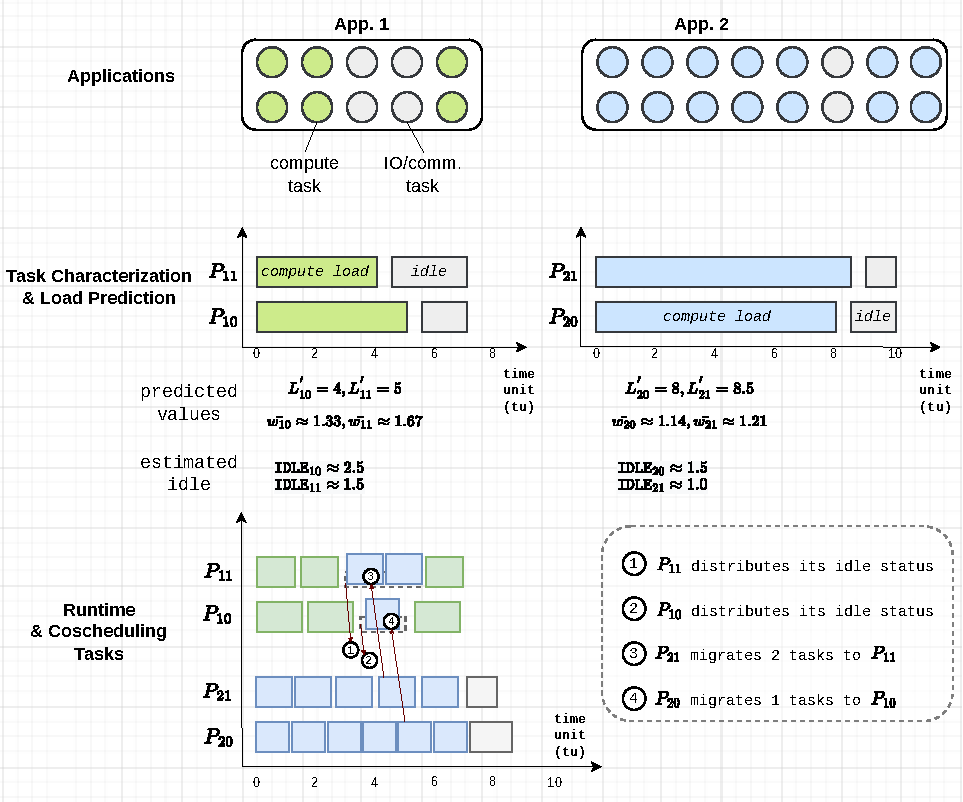
\includegraphics[scale=0.8]{./pictures/padlb_approach/padlb_coscheduling_idea_and_first_usecase.pdf}
	\caption{Co-scheduling strategy and the first use between two CPU applications.}
	\label{fig:proact_coschedule_task_and_first_usecase}
\end{figure}

Second, the procedure \texttt{proact\_coordinate\_TASK()} denotes how tasks are migrated to co-scheduling among the involved processes across different applications. There are two sides to the corresponding operations: one side of processes having idle slots and one side of processes being busy. At Line $9$, $10$, when an idle slot is detected, this information is distributed by the function \texttt{distribute()}. Otherwise, a process checks for receiving idle status from the others. If the idle status is received, a busy process can request offloading tasks (ranging from Line $11$ to $17$). Following that, the busy process waits for a confirmation to proceed with further task offloading if the number of expected tasks and idle slot is matched (indicated by Line $18$, $19$).\\

More intuitively, Figure \ref{fig:proact_coschedule_task_and_first_usecase} demonstrates the operations of Algorithm \ref{alg:proact_coschedule_task}. From top to bottom, we can loosely see three blocks denoted by \textbf{Applications}, \textbf{Task Characterization} \& \textbf{Load Prediction}, and \textbf{Runtime} \& \textbf{Coscheduling Tasks}. The scenario in this figure also illustrates the first use case of our co-scheduling method. In detail, each block is described as follows.

\begin{itemize}
	\item \textbf{Applications}: Two task-based applications are shown in the row of \textbf{Applications}, \texttt{App.1} and \texttt{App.2}. We assume that their tasks include compute tasks and IO/communication tasks. IO/communication tasks are considered idle slots because they are not compute-intensive but waiting for IO/communication. The CPU cores processing these tasks are idle for a period and can be switched to other compute tasks.
	\item \textbf{Task Characterization} \& \textbf{Load Prediction}: We address the stage of profiling tasks and predicting their load values. As illustrated, we give two processes per application; each process spawns multiple threads for executing tasks. Their IDs are indexed by the notation $P_{ij}$, where $i$ and $j$ indicate the index of application and process as mentioned above, e.g., $P_{10}$ indicates process $P_{0}$ belonging to application $1$. Suppose the prediction's results are ready; we have the predicted values of total load ($L^{'}_{ij}$), execution time per task ($w^{'}_{ij}$), and the idle time ($\texttt{IDLE}_{ij}$). For instance, application $1$ is shown with $L^{'}_{10}$, $L^{'}_{11}$, $w^{'}_{10}$, $w^{'}_{11}$, $\texttt{IDLE}_{10}$, and $\texttt{IDLE}_{11}$.
	\item \textbf{Runtime} \& \textbf{Coscheduling Tasks}: We show the illustrated events corresponding to the steps of procedure \texttt{proact\_coordinate\_TASK()} in Algorithm \ref{alg:proact_coschedule_task}. In this use case, \texttt{App.1} has idle slots, \texttt{App.2} is busier with more compute tasks. At the operations \circled{1}, \circled{2}, processes $P_{11}$ and $P_{10}$ of \texttt{App.1} distribute information about their idle status. In principle, after shaking-hand steps to reach an acceptance, process $P_{21}$ and $P_{20}$ of \texttt{App.2} migrates tasks to \texttt{App.1} to take advantage of the idle slots of \texttt{App.1} (shown as the operations \circled{3}, \circled{4}).
\end{itemize}

\begin{figure}[t]
	\centering
	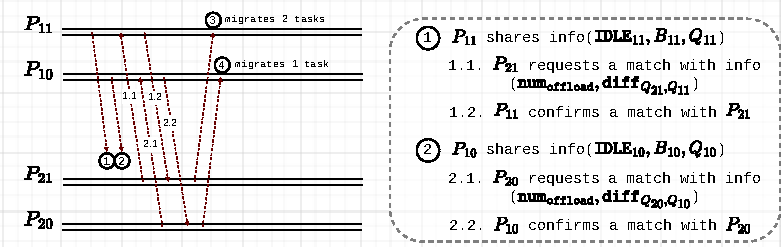
\includegraphics[scale=0.95]{./pictures/padlb_approach/padlb_coscheduling_protocol.pdf}
	\caption{A co-scheduling protocol for exchanging tasks with idle slots.}
	\label{fig:proact_coschedule_protocol}
\end{figure}

The operations \circled{1}, \circled{2}, \circled{3}, \circled{4} are detailed in Figure \ref{fig:proact_coschedule_protocol}. We have hand-shaking steps before tasks are offloaded. To ease the coordination between the processes of two applications, we distribute idle status associated with its estimated value, bandwidth information ($B$), and the current status of the queue. Bandwidth $B$ can be measured in advance and averaged gradually from the information exchange of previous steps. We attach it to calculate transmission time before offloading tasks. Furthermore, we need information about the current queue length to check how many remaining tasks there are and the queue lengths between the idle and busy processes. For example, $P_{11}$ distributes a message of $\texttt{IDLE}_{11}$, $B_{11}$, $Q_{11}$ at operation \circled{1}. On the side receiving idle status, the arrived information is checked first with the difference in queue length to ensure that there are still available tasks for migration. Then, we calculate a suitable number of tasks that should be offloaded from the busy process based on $\texttt{IDLE}$. The calculated amount of tasks should not exceed the capability of average bandwidth $B$ through a ratio, $\frac{\texttt{IDLE}\times B}{\texttt{data\_size}/task}$. Thereby, we can calculate how many tasks should fit the gap. For example, $P_{21}$ sends a request to match with $P_{11}$ at $1.1$ after calculating the number of available tasks. If $P_{11}$ agrees, it sends a confirmation message at $1.2$, and tasks are offloaded afterward. The selected victim for co-scheduling tasks during an idle period is ranked and prioritized from the sorted array of $\texttt{IDLE}^{'}$.\\

Several realistic HPC applications can represent the use case shown in Figure \ref{fig:proact_coschedule_task_and_first_usecase}. They have become more popular with large-scale simulations, such as environment issue simulations. More importantly, these applications must run with various scenarios and long-term tuning of the parameters for an optimal performance setup in HPC clusters. Hence, the idea of co-scheduling tasks in this method can be beneficial when one program has available idle slots, which are long enough to be replaced by tasks from another program. Our method can make both programs efficient and achieve better computing resource utilization. \\

For today's aspects with ML/DL applications, we illustrate another use case in Figure \ref{fig:proact_coschedule_second_usecase}. The x-axis shows time progress, while the y-axis highlights each application's processes and GPU region. The top is application $1$ (\texttt{App.1}), and the bottom is application 2 (\texttt{App.2}). Vertically, the process labels imply tasks executing on the CPU side (\texttt{CPU compute task}), while the GPU labels imply tasks executing on the GPU side (\texttt{GPU compute task}), and the blocks with dashed borders indicate idle slots. The main idea for applying our method to this use case includes:
\begin{itemize}
	\item An application has two types of tasks, \texttt{CPU compute task} and \texttt{GPU compute task}. Assuming when GPU tasks on an application are running, the CPU side is idle.
	\item When the CPU side of an application is idle, CPU tasks from another application can be migrated to fill the idle slots.
\end{itemize}

This use case becomes more familiar with heterogeneous architectures, i.e., CPU-GPU. In Figure \ref{fig:proact_coschedule_second_usecase}, we assume a distributed memory system of CPU-GPU nodes. We can share tasks during idle slots if tasks are well-defined.\\

% As illustrated in Figure \ref{fig:proact_coschedule_second_usecase}, there are also two applications, but tasks include CPU-GPU tasks and idle slots for waiting data movement between both sides.  Similarly, tasks from the busy side are migrated to the idle side with an estimation of communication overhead. \\

\begin{figure}[t]
	\centering
	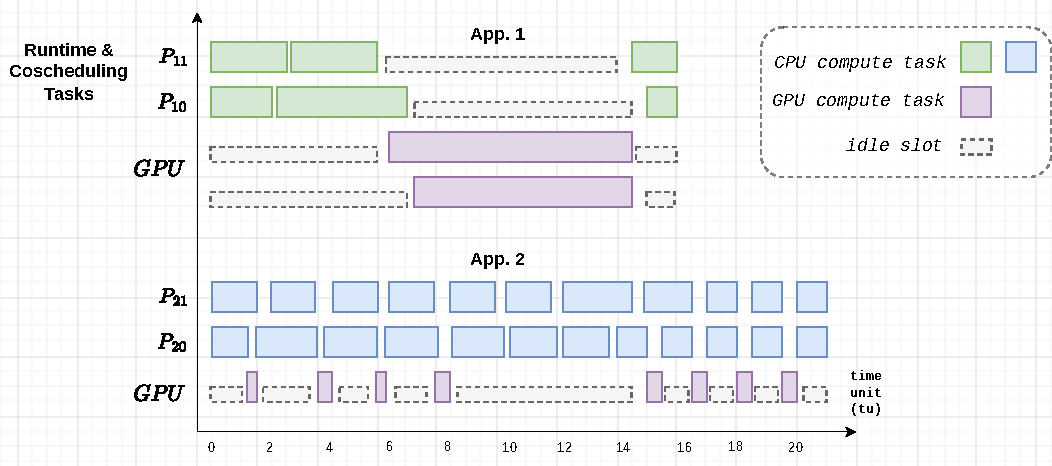
\includegraphics[scale=0.85]{./pictures/padlb_approach/padlb_coscheduling_second_usecase.pdf}
	\caption{The second use case of proactive coscheduling tasks.}
	\label{fig:proact_coschedule_second_usecase}
\end{figure}

In the following chapters, we will show the implementation of our two methods and this extension. Significantly, with this extension for co-scheduling tasks, we cannot interfere with the execution of jobs in HPC clusters due to permission. Therefore, the experiments are emulated by defining different tasks in an executable, representing multiple applications that run simultaneously. Different tasks from different applications are in the same executable. For example, there is a whole job executing on $4$ compute nodes, where two nodes will host the first application with its tasks, and the remaining nodes will host the second application. In such a submitted job, the two applications run simultaneously, enabling MPI to provide the same communication environment between them.

% One advantage of task-based applications is an abstraction of task definition, which points to the code and data. Therefore, it is feasible to profile the characteristics of tasks, e.g., inputs, outputs, that we can combine with system information, e.g., core frequencies, performance counters, to predict the load values. 

